% !TEX encoding = UTF-8 Unicode
\documentclass[convert={density=300,size=1000x700,outext=.png}]{standalone}
\usepackage{tikz}
% \usepackage[active,tightpage,psfixbb]{preview}
\usepackage{tipa,dingbat}
% \PreviewEnvironment{pgfpicture}
% \setlength\PreviewBorder{2pt}
\usetikzlibrary{positioning, shapes}



\begin{document}
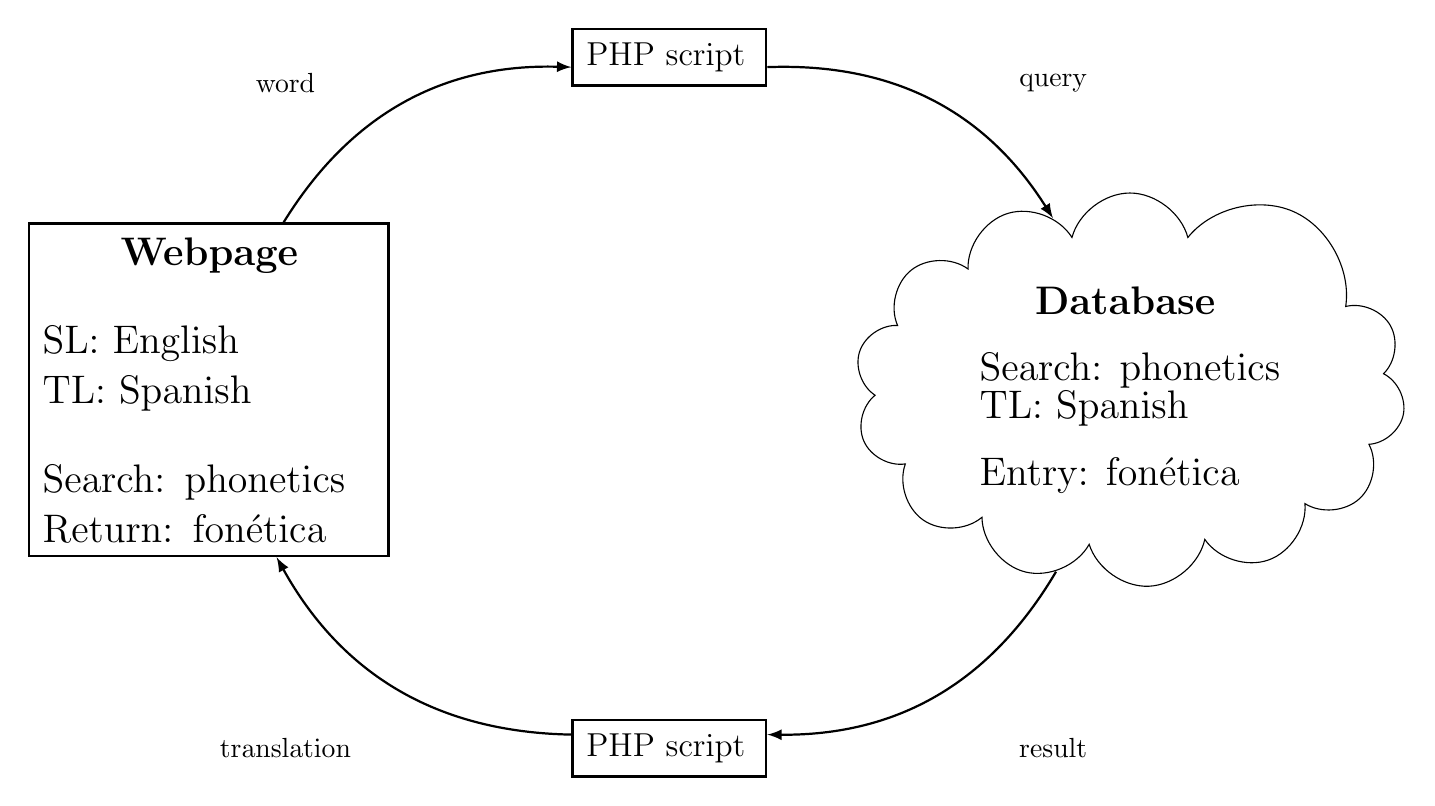
\begin{tikzpicture}[scale=.65]

% \draw[help lines] (0,0) grid (38,31);

\tikzstyle{gbox1}=[draw=black, thick,shape=rectangle,inner sep=5pt,
text width=12em, font=\Large];
\tikzstyle{gbox2}=[draw=black, thick,shape=rectangle,inner sep=5pt,
text width=6em, font=\large];
\tikzstyle{gbox3}=[draw=black, thick,shape=rectangle,inner sep=5pt,
text width=6em, font=\large];

\node[gbox1] (a1) at (1,15) {\hspace{2em}\textbf{Webpage} \\ \vspace{1em} SL: English \\ TL: Spanish \vspace{1em} \\ Search: phonetics \\ Return: fon\'etica};
\node[gbox2] (a2) at (10,21.5) {PHP script};
\node[cloud, cloud puffs=13.7, cloud ignores aspect, minimum width=7cm, minimum height=5cm, align=left, draw] (a3) at (19,15) {\hspace{2em}\Large{\textbf{Database}} \\ \phantom{hi} \\ \Large{Search: phonetics} \\ \Large{TL: Spanish} \\ \phantom{hi} \\ \Large{Entry: fon\'etica}};
\node[gbox3] (a4) at (10,8) {PHP script};

\node at (2.5,21) {word};
\node at (17.5,21) {query};

\node at (17.5,8) {result};
\node at (2.5,8) {translation};

% lines
\draw [-latex, thick] (a1) to[bend left=30] (a2) ;
\draw [-latex, thick] (a2) to[bend left=30] (a3) ;
\draw [-latex, thick] (a3) to[bend left=30] (a4) ;
\draw [-latex, thick] (a4) to[bend left=30] (a1) ;






\end{tikzpicture}
\end{document}